\documentclass[tikz,border=8pt]{standalone}

\usepackage{amsmath}
\usetikzlibrary{arrows.meta,positioning,calc}

\definecolor{tmfblue}{HTML}{3575A7}
\definecolor{tmfteal}{HTML}{3F9483}
\definecolor{tmforange}{HTML}{D98254}
\definecolor{tmfgray}{HTML}{65717E}

\begin{document}
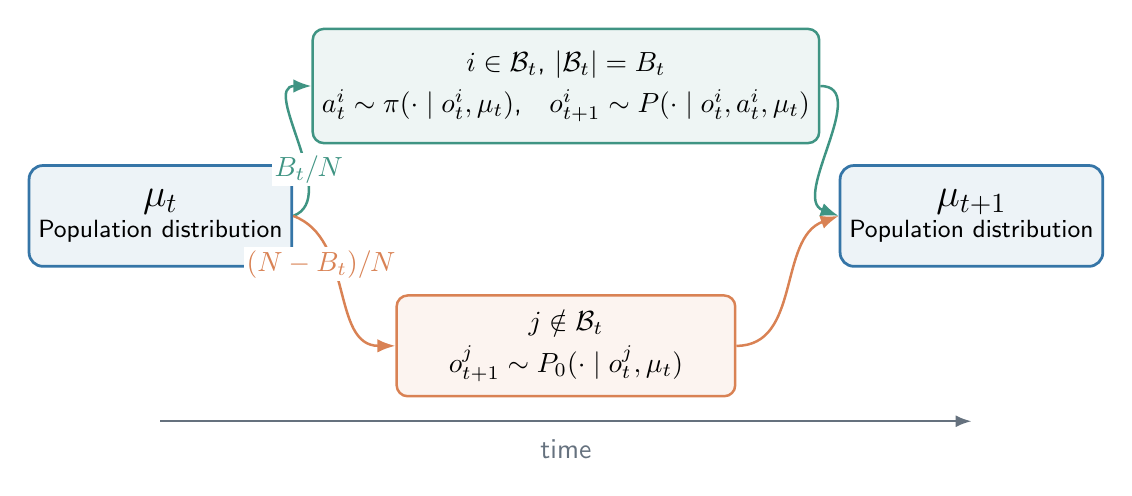
\begin{tikzpicture}[
    font=\sffamily,
    >=Latex,
    state/.style={
        draw=tmfblue,
        fill=tmfblue!9,
        rounded corners=5pt,
        minimum width=2.15cm,
        minimum height=1.28cm,
        align=center,
        line width=1pt
    },
    active/.style={
        draw=tmfteal,
        fill=tmfteal!9,
        rounded corners=4pt,
        minimum width=4.3cm,
        minimum height=1.45cm,
        align=center,
        line width=0.9pt
    },
    other/.style={
        draw=tmforange,
        fill=tmforange!9,
        rounded corners=4pt,
        minimum width=4.3cm,
        minimum height=1.28cm,
        align=center,
        line width=0.9pt
    },
    flow/.style={-{Latex[length=2.3mm]},line width=0.9pt}
]

% Current and next population distributions
\node[state] (mut) at (0,0) {\Large $\mu_t$\\[-1pt]\small Population distribution};
\node[state] (munext) at (10.3,0) {\Large $\mu_{t+1}$\\[-1pt]\small Population distribution};

% Two components of the TMF update
\node[active] (active) at (5.15,1.65) {
    $i\in\mathcal B_t$, $|\mathcal B_t|=B_t$\\[3pt]
    $a_t^i\sim\pi(\cdot\mid o_t^i,\mu_t)$,\quad
    $o_{t+1}^i\sim P(\cdot\mid o_t^i,a_t^i,\mu_t)$
};

\node[other] (other) at (5.15,-1.65) {
    $j\notin\mathcal B_t$\\[3pt]
    $o_{t+1}^j\sim P_0(\cdot\mid o_t^j,\mu_t)$
};

% Split from mu_t
\draw[flow,tmfteal] (mut.east) to[out=20,in=180]
    node[pos=0.20,above=3pt,fill=white,inner sep=1pt,text=tmfteal] {$B_t/N$} (active.west);
\draw[flow,tmforange] (mut.east) to[out=-20,in=180]
    node[pos=0.20,below=3pt,fill=white,inner sep=1pt,text=tmforange] {$(N-B_t)/N$} (other.west);

% Merge into mu_{t+1}
\draw[flow,tmfteal] (active.east) to[out=0,in=160] (munext.west);
\draw[flow,tmforange] (other.east) to[out=0,in=-160] (munext.west);

% Time direction
\draw[-{Latex[length=2mm]},tmfgray,line width=0.7pt]
    ($(mut.south)+(0,-1.95)$) -- node[below=3pt] {time} ($(munext.south)+(0,-1.95)$);

\end{tikzpicture}
\end{document}
